%!TEX root = ../Single-Song.tex
\beginsong{Trollträume}[wuw={Isabel Eisenträger, Kathrin Bernhardt, Christian Bruns}, jahr=2016]

\beginverse
\endverse
\centering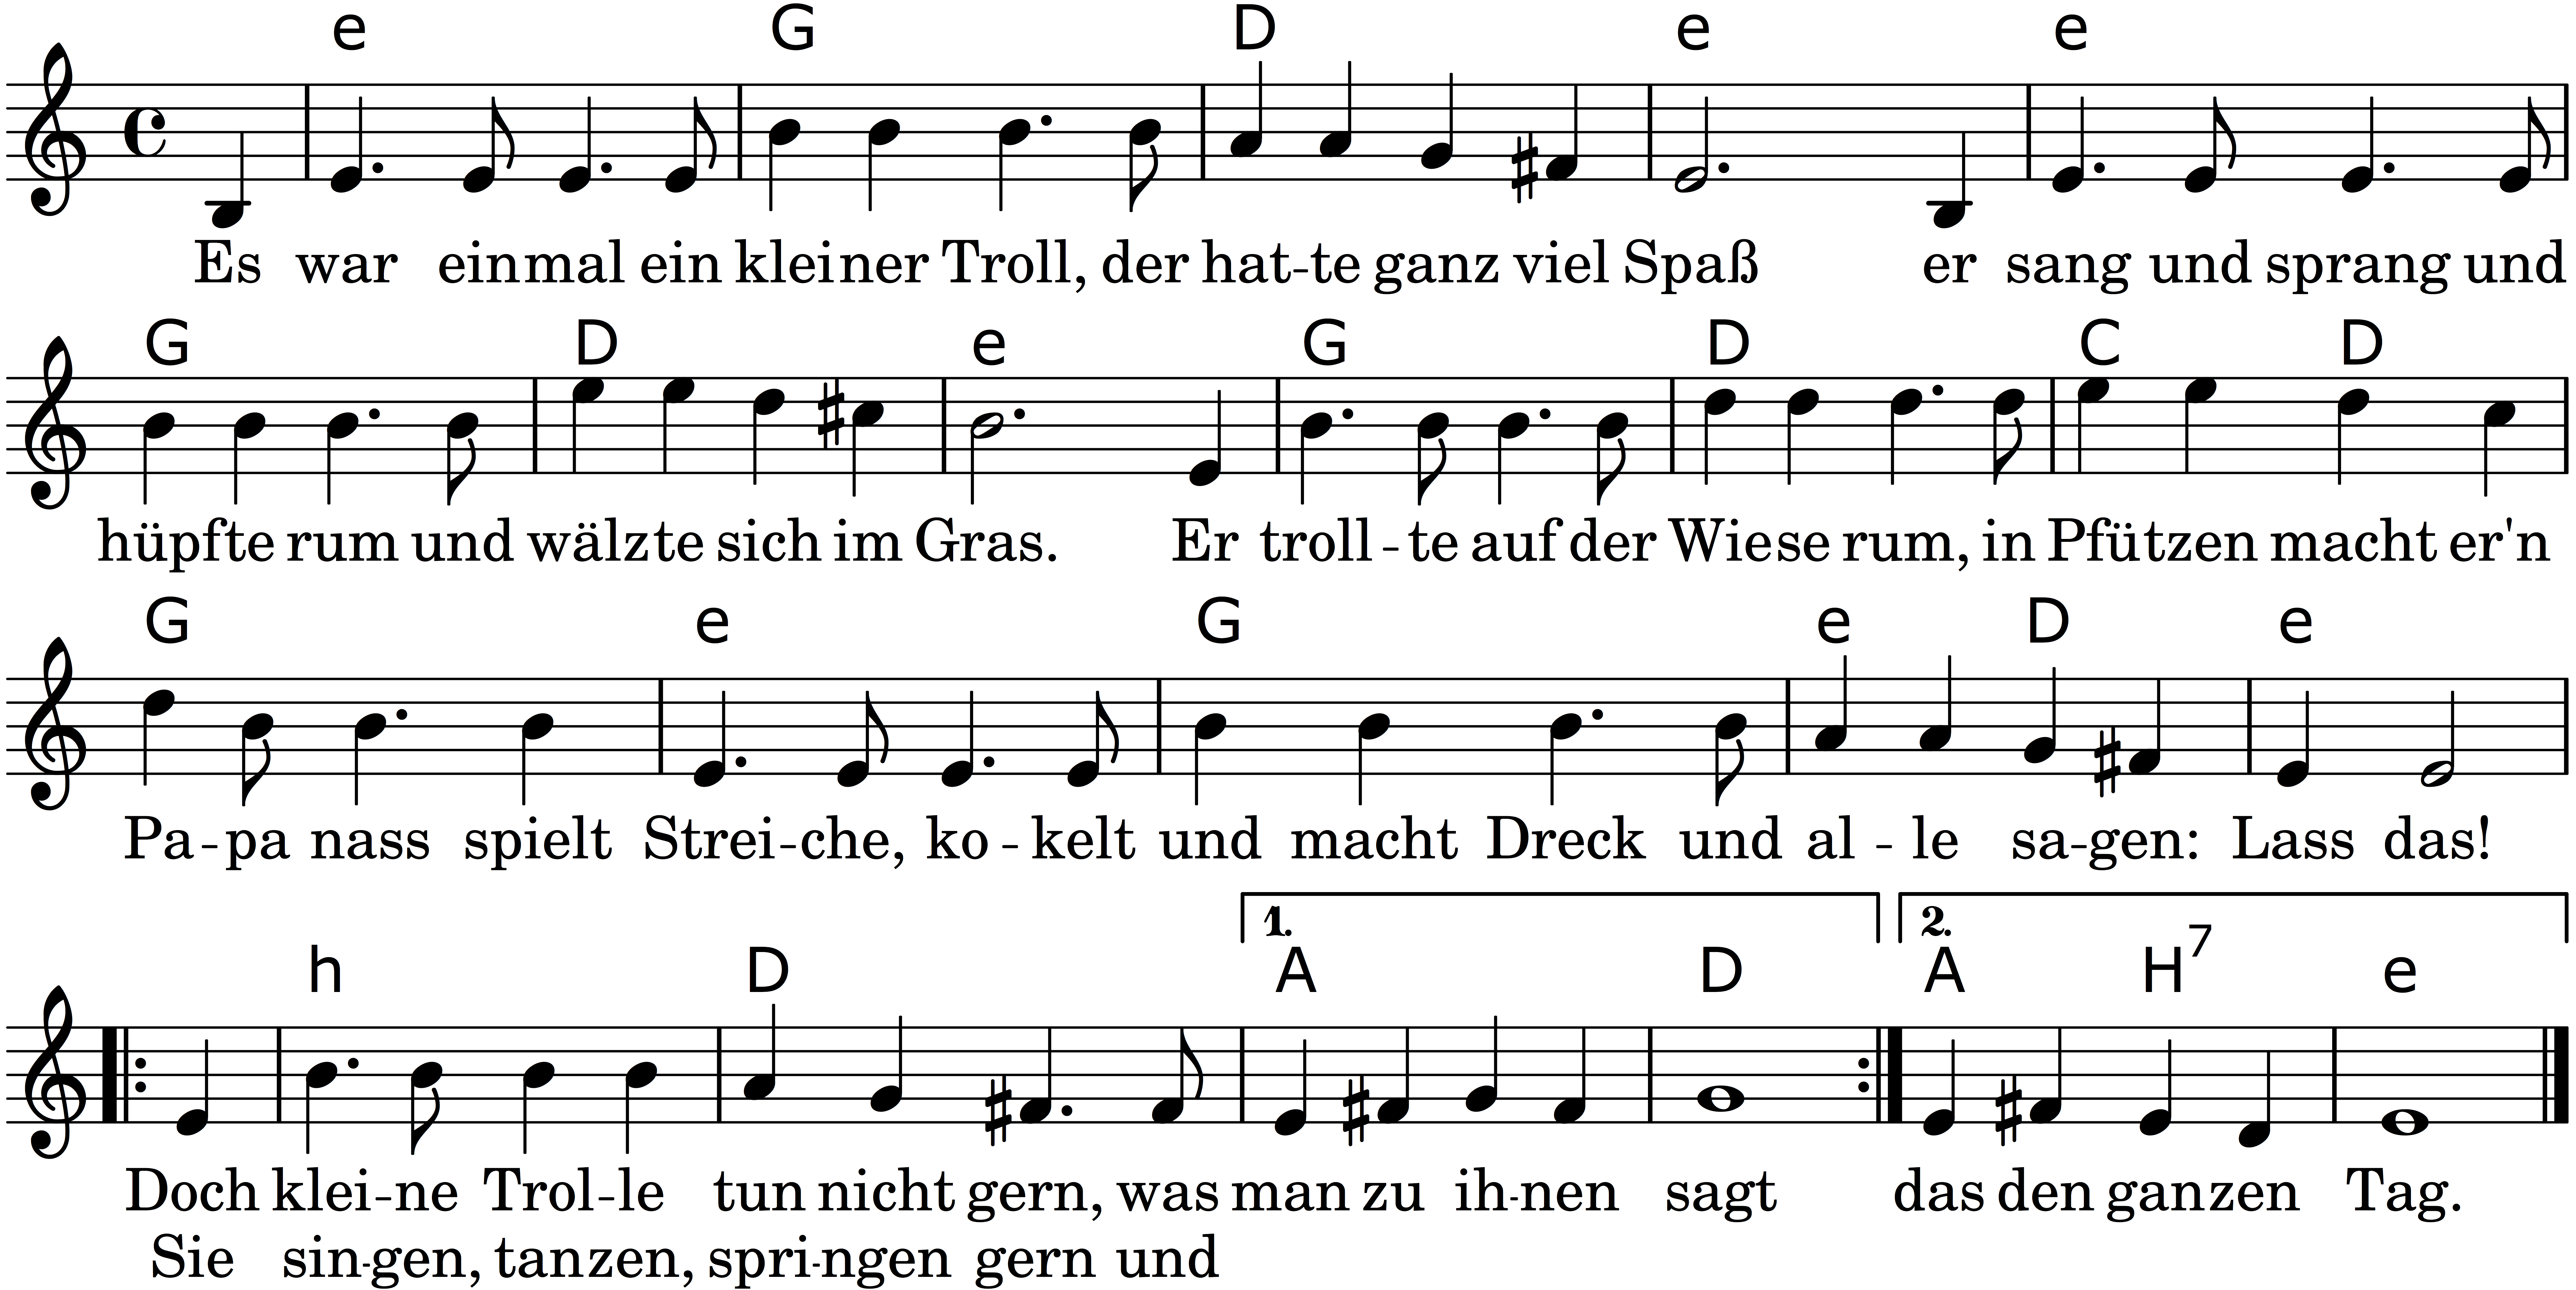
\includegraphics[width=1\textwidth]{Noten/Trolltraeume.png}

% \beginverse
% Es \[Em]war war ein mal ein \[G]kleiner Troll, der \[D]hatte ganz viel \[Em]Spaß,
% er \[Em]sang und sprang und \[G]hüpfte rum um \[D]wälzte sich im \[Em]Gras.
% Er \[G]trollte auf der \[D]Wiese rum, in \[C]Pfützen \[D]macht er'n \[G]Papa nass,
% spielt \[Em]Streiche, kokelt \[D]und macht Dreck und \[Em]alle \[D]sagen: \[Em]Lass das!
% \endverse
%
% \beginchorus
% Doch \[Hm]kleine Trolle \[D]tun nicht gern, was \[A]man zu ihnen \[D]sagt.
% Sie \[Hm]singen, tanzen, \[D]springen gern und \[A]das den \[Hm7]ganzen \[Em]Tag.
% \endchorus

\beginverse
Der \[Em]kleine Troll liegt \[G]müd' im Bett und \[D]träumt er sei schon \[Em]zwölf,
er \[Em]will nun nur noch \[G]tanzen geh'n ins \[D]Bett geh'n erst um \[Em]ölf.
\[G]Hausaufgaben, \[D]Mathe schwänzen (und) \[C]Trollbier \[D]gibt's vom \[G]Fass.
Vi\[Em]sionen haben, \[G]Welt verändern und \[Em]alle \[D]sagen: \[Em]Lass das!
\endverse

\beginchorus
Doch \[Hm]kleine Trolle \[D]tun nicht gern, was \[A]man zu ihnen \[D]sagt.
Sie \[Hm]singen, tanzen, \[D]springen gern und \[A]das den \[H7]ganzen \[Em]Tag.
\endchorus

\beginverse
Als ^großer Troll hat ^er gelernt, dass ^er dies lieber ^lässt.
Er ^spielt und singt und ^tanzt nicht gern, geht ^niemals auf ein ^Fest.
Bau^sparverträge, ^keine Zeit, schaut ^nie zu ^tief ins ^Glas
und ^seinem Kind, das ^Spaß nur hat, sagt ^er nur ^ganz streng: ^Lass das!
\endverse

\beginchorus
Doch \[Hm]kleine Trolle \[D]tun nicht gern, was \[A]man zu ihnen \[D]sagt.
Sie \[Hm]singen, tanzen, \[D]springen gern und \[A]das den \[H7]ganzen \[Em]Tag.
\endchorus

\beginverse
Der ^kleine Troll, der ^wacht nun auf, hat ^Schweiß noch im Ge^sicht.
Was ^für ein Schrecken, ^großer Graus, so ^werden will ich ^nicht.
Drum ^sing und spiel und ^tanz ich gern und ^habe ^ganz viel ^Spaß.
Und ^wenn ich einmal ^Papa bin will ^ich nicht ^sagen: ^Lass das!
\endverse

\beginchorus
Doch \[Hm]kleine Trolle \[D]tun nicht gern, was \[A]man zu ihnen \[D]sagt.
Sie \[Hm]singen, tanzen, \[D]springen gern und \[A]das den \[H7]ganzen \[Em]Tag.
\endchorus

\endsong
\beginscripture{}
Das Lied wurde im Jahr 2016 vom VCP Singekreis Mitteldeutschland anlässlich des Hamburger Singewettstreits (HaSiWe) 2017 geschrieben und den ersten Platz in der Kategorie \emph{Singekreise} belegt. Der Singekreis belegte mit diesem Lied auf dem VCP Bundeslager 2017 ebenfalls den ersten Platz.
\endscripture

\begin{intersong}

\end{intersong}